\subsection{Tracking Overview}
The reconstruction program must reconstruct, on an event-by-event basis, the raw data coming from either
simulation or the detectors to provide physics analysis output such as track parameters and particle
identification. Charged particle tracking is separated into the reconstruction of tracks in the central
(Silicon and Micromegas Vertex Trackers) and forward (Forward Micromegas Tracker and Drift
Chambers) detectors. The forward region covers the angular range from $5^\circ$ to $40^\circ$, while
the Central Detector covers approximately $40^\circ$ to $135^\circ$. In the central region a 5~T
solenoidal magnetic field bends charged tracks into helices, while forward-going tracks are bent by a
$\sim$2~T toroidal magnetic field. For both systems, track reconstruction comprises algorithms for
pattern recognition and track fitting. Hit objects, corresponding to the passage of a particle through a
particular detector component, require the transformation of an electronic signal into a location of the
track's position in the detector sub-system geometry. A hit is thus a geometric object, for example, a
line segment. These objects then form the input to the pattern recognition algorithms. This first step
involves the identification of clusters of hits and the determination of the spatial coordinates and
corresponding uncertainties for hits and clusters of hits. At the pattern recognition stage, hits that are
consistent with belonging to a trajectory (i.e. track) are identified. This set of hits is then fit to the
expected trajectory with their uncertainties, incorporating the knowledge of the detector material and
the detailed magnetic field map.

CLAS12 has a unique magnetic field configuration that involves tracking though both a solenoidal and toroidal field. Tracks reconstructed in the forward detector are fit in the forward tracking detectors and subsequently swam to the beam line through both fields.  A view of the field intensities in the $(z,x)$ plane and overlap region for the torus and solenoid fields is shown in Fig.~\ref{fig:fields}.

\begin{figure}
\centering
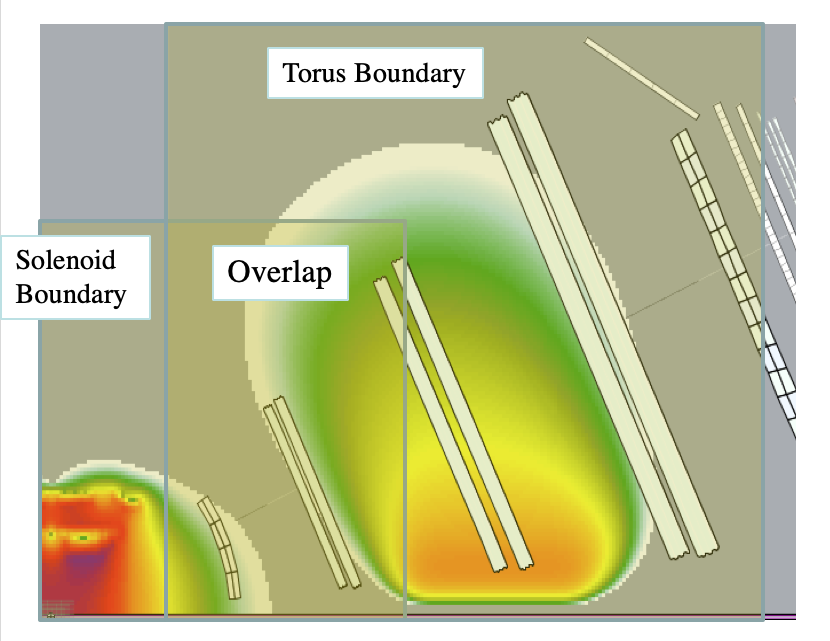
\includegraphics[width=0.5\textwidth]{pics/Bfields.png}
\caption{Event display of the CLAS12 magnetic fields. 
}
\label{fig:fields}
\end{figure}

\subsection{Forward Tracking}

\subsubsection{Hit Reconstruction}

The Drift Chamber (DC) wire hit information is given by the wire geometrical location and the drift time
to the wire. Track-dependent corrections to the hit, such as left-right ambiguity and time-walk must then
be performed. 
Pattern recognition for the DC is priori done using only wire position information and searching for groups of hits forming clusters.  This portion of the algorithms is called ``hit-based'' tracking.  In hit-based
tracking, a hit is defined as a wire with a recorded signal.  No timing information is incorporated at the
preliminary stage of the reconstruction.  
After a ``hit-based''  track has been found, corrections to the raw TDCs of the hits on track resulting from the propagation time along the hit wire, the signal time of flight, the event start time and the cable delays are applied to determine the hit time.  A distance of closest approach (DOCA) to the hit wire is estimated from the time.  At this stage the tracking is redone using the calculated DOCAs in order to fit the track (see Fig.~\ref{fig:docas}.  This portion of the DC reconstruction phase is called ``time-based'' tracking.  The calibration parameters entering in the function used to convert distance to time that is inverted in reconstruction (see Ref. DC paper) are extracted from the distance of local fits to the DOCAs using a linear function to the wire position. 

\begin{figure}
\centering
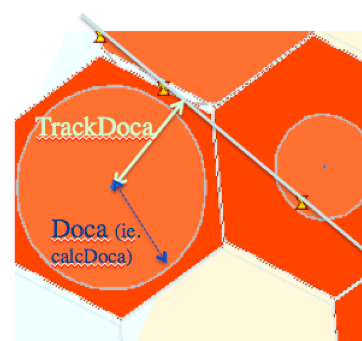
\includegraphics[width=0.2\textwidth]{pics/dcPattern10.png}
\caption{
Illustration of DOCA computed from the corrected time and of the distance from the wire to the track (TrackDoca).
}
\label{fig:docas}
\end{figure}

In hit-based
tracking, uncorrelated hit noise in the DC are identified by a Simple Noise
Removal (SNR) algorithm and rejected. SNR stores all the data for a drift chamber layer (112 sense wires)
bitwise in an extended 128-bit word, with "set" bits corresponding to hits. The algorithm is configured
through parameters specifying the maximum tilt of a track segment and the number of missing layers
allowed in the formation of a segment. Using bitwise operations on the extended words, the algorithm
essentially operates as a parallel processor on all 112 sense wires in layer. This parallelism precludes the
need of a wire for-loop, enabling the algorithm to run in a negligible fraction of the total time for
reconstruction. More to the point, SNR actually saves time by reducing the combinations that must be
explored in the pattern-recognition phase of the ensuing track-finding.
An illustration of the SNR hit categorization in the DC is displayed in Fig.~\ref{fig:snr}.
\begin{figure}
\centering
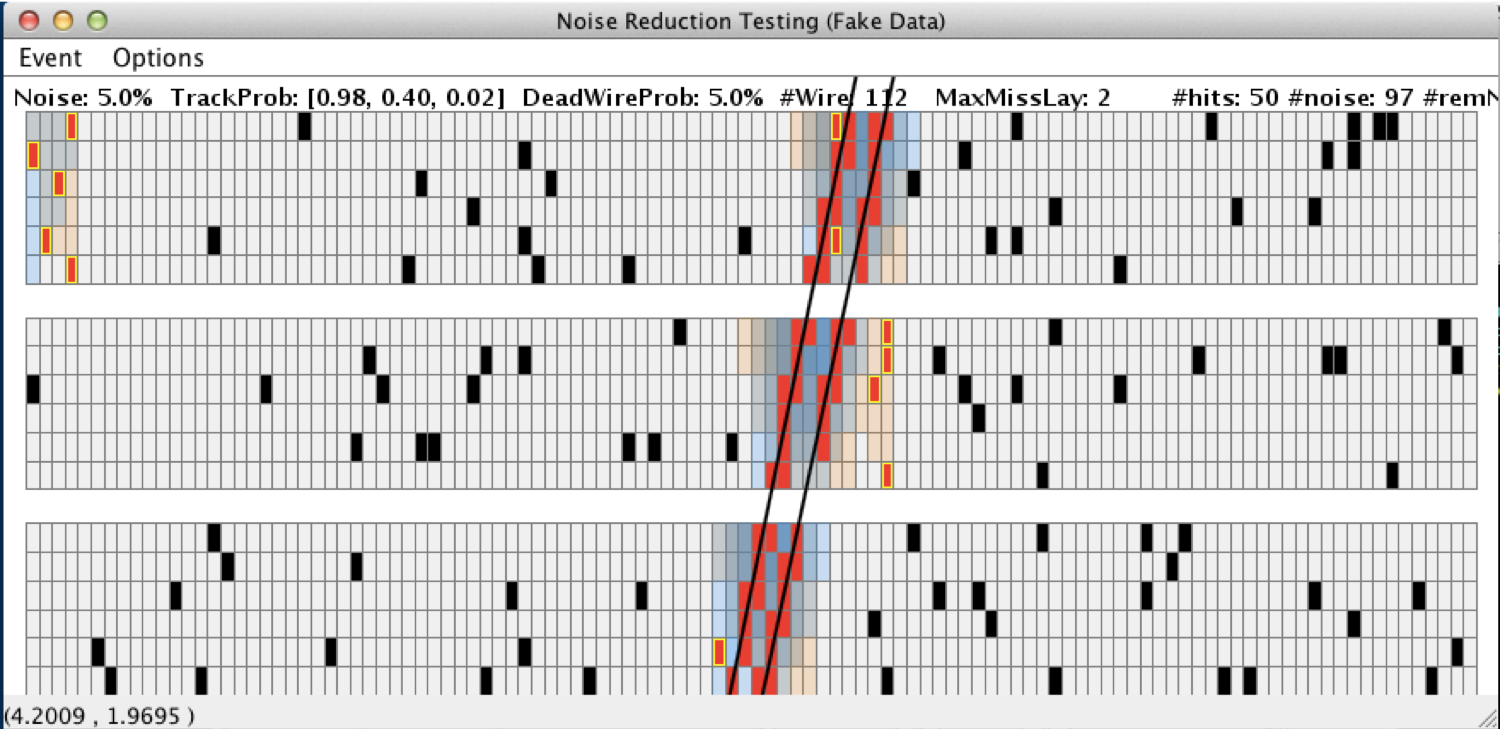
\includegraphics[width=0.48\textwidth]{pics/dcPattern9.png}
\caption{
Illustration of DC hits categorized by the SNR algorithm.  
Black hits are identified as noise and discarded.
Red hits are saved for further evaluation by the subsequent hit selection algorithms. 
Red hits with yellow frames are saved noise (false alarms).  Shaded areas correspond to 
possible clusters.  The darker shades correspond to a higher quality factor, hence a higher probability for hits on track.
}
\label{fig:snr}
\end{figure}

\subsubsection{Hit Clustering}
The hits remaining after the SNR
algorithm are grouped into clusters.
Clusters are groups of adjacent hits in a group of 6 layers forming a DC superlayer.  There can be at most
two hits in a layer, forming a ``double-hit''~\footnote{An additional hit in a layer is mostly out of time and has 
a drift time that when converted to a drift distance exceeds the cell size. }  However, up to four layers can be missing in a superlayer
when attempting to form a cluster.  This is to reduce tracking inefficiencies resulting from possible wire malfunctions or
intrinsic inefficiencies. It was found that using 4 out of 6 layers to form a cluster is good enough
to determine the cluster shape which is subsequently used in tracking to determine the track trajectory. 
\begin{figure}
\centering
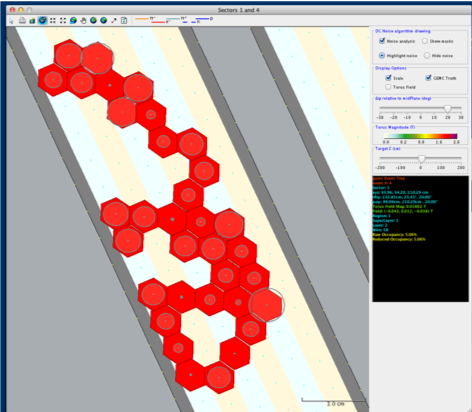
\includegraphics[width=0.4\textwidth]{pics/elooper.png}
\caption{
Illustration of typical noise patterns in the DC displayed with the CLAS12 Event Display (CED). 
The hits shown in the display correspond to electrons from a MC sample.
}
\label{fig:eloop}
\end{figure}

Additional ``noise rejection'' algorithms are applied to the clusters to remove spurious hits
that do not come from a real track. 
So-called ``curlers'' patterns as show in Fig~\ref{fig:eloop} are typical for low energy electrons  in the DC.   So a pruning algorithm was designed to remove them at an early stage of the reconstruction. The  algorithm is a counting method of the number of contiguous hits in a layer of a superlayer.  In Figs.~\ref{fig:eloop} and ~\ref{fig:strings} we also see another typical noise pattern that looks like horizontal ``strings'' of hits along a layer.  The algorithm was developed following  the observation that high-momentum tracks from hadrons typically cross the superlayers at a large angle,
while ``curlers'' from low-momentum background follow curling trajectories with a significant part of the
pattern being along layers.
Subsequent algorithms  are employed for resolving overlapping segments.   
\begin{figure}
\centering
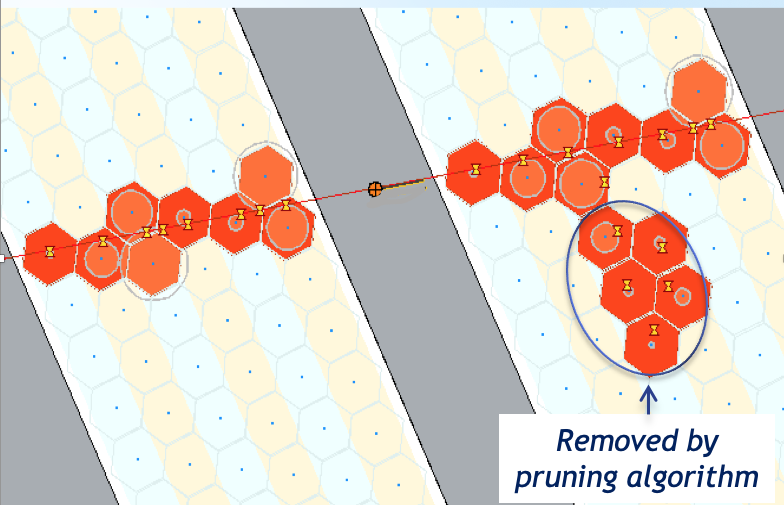
\includegraphics[width=0.4\textwidth]{pics/dcPattern2.png}
\caption{
Illustration is hits rejected by the pattern recognition algorithm in a MC sample corresponding to electron tracks generated at 4.5 GeV at the center of the sector ($\phi = 0\deg$ with a polar angle of $10\deg$. 
The circles superimposed on top of the DC cells indicate the DOCAs computed from the fully corrected times.  The yellow hourglass symbols show the simulated track positions along the trajectory.   
The algorithm looks for ``strings'' of hits such as shown in the the third column of hits in the right-most superlayer in the figure.  
In this instance, the middle hit would be rejected, leaving a set of four attached hits which would subsequently be rejected since they would no longer be attached to the main cluster. 
}
\label{fig:strings}
\end{figure}


Overlapping segments are produced when the trajectories of tracks cross each other
or when the tracks are almost parallel and very close to each other in a given region.
A Hough transform is employed to find hits on a line in the cluster which allows splitting the cluster into
segments.  The resulting trimmed clusters are then fit to a straight-line hypothesis, and those hits with
acceptable residuals are kept and identified collectively as a ``track segment''. An illustration of the Hough Transform cluster selection algorithm is shown in Fig.~\ref{fig:hough}.

Subsequent hit pruning algorithms are employed at ``time-based'' level.  
Figure~\ref{fig:dcsegs} illustrates the selected hits belonging to a cluster (orange) and the hits
rejected by the noise-finding algorithms.

\subsubsection{Pattern Recognition}
Fits to the segments with a linear function are a preliminary step to estimating
a track trajectory. Track parameters are estimated in the local coordinate system of the chamber sector from
this trajectory.

\begin{figure}
\centering
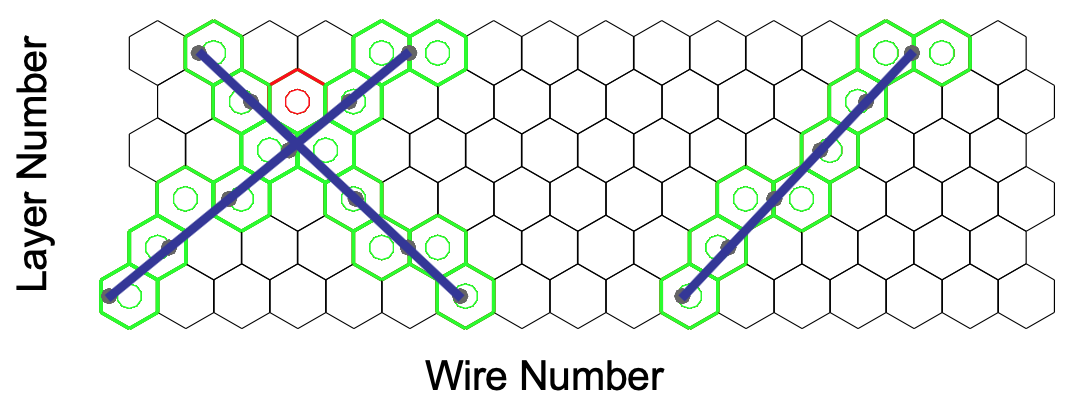
\includegraphics[width=0.45\textwidth]{pics/dcPattern14.png}
\caption{
Illustration of selected clusters (left-most selected hits with superimposed lines) using a Hough Transform.  Two track segments cross each other.  The hits are separated into cluster candidates and fit using a local coordinate system as a function of layer and wire number.  The selection is done without employing timing information. 
}
\label{fig:hough}
\end{figure}
Using the wire direction in a given superlayer along with the line fit to a segment in that superlayer, a plane can be constructed.
Thus pairs of segments in
neighboring superlayers within one chamber (with superlayers of $\pm$6$^\circ$ stereo angle) represent the
intersection of two planes, that is a line whose coordinates are evaluated midway between the two
superlayers, and is a 6-dimensional object (x,y,z and 3 angles) which we call a ``cross''.
A segment slope coincidence algorithm is used to match neighboring segments in a region (see
Fig.~\ref{fig:dcsegs}).  Selection cuts are subsequently applied on the
reconstructed cross to ensure that it is within the fiducial sector volume within resolution.

\begin{figure}
\centering
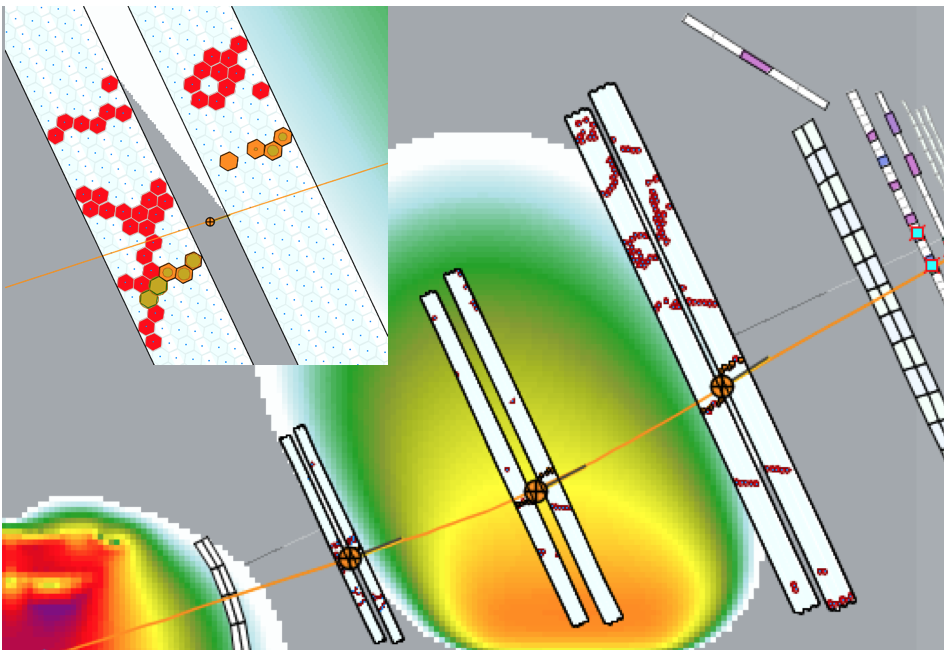
\includegraphics[width=0.4\textwidth]{pics/dcPattern13.png}
\caption{
Illustration is hits (red hexagons) rejected and accepted (orange hexagons) by the pattern recognition algorithm in a MC.  
The red cells correspond to hits not rejected by the SNR algorithm.  The circles represent the calculated DOCAs.  The superimposed lines show the local fits to the DOCAs.  The filled circle in the middle of the two superlayers represents the 3-dimentional point (i.e. ``cross'') obtained from the local fits to the DOCAs taking into account the direction along the wires.
The offset between the segments composing the cross comes from the projection at the $y=0$ plane (midplane).
The cluster shown on the right-most superlayer is an example of a ``looper'' and shows how this category of cluster has the potential to bias the track.  The second cluster used to form the cross yield an incorrect slope resulting from a wrong hit used in the fit.  Subsequently, the ``looper'' searcher algorithm rejects the entire cluster and only the first cluster is used to fit the track.  The fitted track trajectory is represented by the orange line. 
The upper figure is a zoomed view into the track trajectory in region 1.
}
\label{fig:dcsegs}
\end{figure}


An additional  pattern reconstruction algorithm  matches segments within even and odd superlayers, respectively, to form
a track candidate where an entire superlayer can be missing.  The matching algorithm returns an estimates of where the missing
superlayers hits should be and forms a pseudo-segment from the wire locations corresponding to these hits.  Subsequently
a pseudo-cross is formed using the pseudo-segment and the neighboring reconstructed segment in that region.

The first stage of
pattern-recognition consists of finding a track candidate, from a set of 3 crosses (one each in R1, R2 and R3) that
are fit to a parabolic functional form to give us a ``track candidate''.
Using the parameters of the parabolic function between the first and the third cross and obtaining the magnetic field
intensity at each step along this trajectory we obtain an estimate for $\int B dl$.
From the local angles of the crosses in the $x-z$ plane for R1 ($\theta_1$) and R3 ($\theta_3$) we estimate the track momentum ($p$)
and the particle's charge ($q$),
as follows:
\begin{equation}\frac{q}{p} = \frac{\theta_3 - \theta_1}{v\int{B dl}},\end{equation} where the angles are in radians, the magnetic field
intensity ($B$) is in Tesla, and the pathlength ($dl$) in cm.
The conversion factor  $v = 0.002997924580 (GeV/c) T^{-1} cm^{-1}$  corresponds to the speed of light.
The cross position and angles in region 1 together with the
momentum and the charge provide all the necessary information to define the track parameters at a given location in the detector,
and therefore to start track fitting.


\subsubsection{Track Fitting}
The output of the pattern recognition
is a seed with initial parameters used to start the track propagation from one measurement site to the next in the fit.
Track fitting uses a Kalman Filter method with a 5-parameter track representation ($x$, $y$, $tx$, $ty$, $q$/$p$), defined
in a local coordinate system with the z-axis perpendicular to the chambers wire planes; where $q$ is the
track charge, $tx=px$/$pz$,
$ty=py$/$pz$, with $px,py,pz$ resenting the $x,y,z$ components of the track momentum in that (analysis) frame.
In the analysis frame the state vector (representing the track parameters) and the measurement are defined at each layer
at which there is a hit on track.
Hence, as in ref~\cite{spiri} we can express the equations of motion of the track in the torus field
and the propagation of the state vector covariance matrix as derivatives with respect to $z$.
In the drift chambers, the magnetic field components are mostly along the $y$ coordinate in the analysis frame.
The trajectory of the particle in the analysis frame is given by the following equations:

\begin{eqnarray*}
%\systeme{
dx/dz  &=& tx, \\
dy/dz  &=&  ty, \\
dtx/dz &=& q \cdot v \cdot \sqrt{1 + {t_x}^2 + {t_y}^2}\cdot [t_y\cdot (t_x B_x + B_z)\\ &-& (1 + {t_x}^2 ) B_y], \\
dty/dz  &=&  q \cdot v \cdot \sqrt{1 + {t_x}^2 + {t_y}^2}\cdot [-t_x\cdot (t_y B_y + B_z) \\&+& (1 + {t_y}^2 ) B_y], \\
q  &=&  q_0,
%}
\end{eqnarray*}


where, and the initial values at the initial plane $z = z_{0}$ are
$x = x_{0}, y = y_{0}, t_x = t_{x0}, t_y = t_{y0}, q = q_{0}$.

we solve the above equations
numerically using a fourth order Runge-Kutta integration method in order to propagate the state vector from
the drift chamber plane at $z_{0}$ to the next one at $z$.  The state covariance matrix is propagated along with it
by computing the Jacobian matrices as in ref~\cite{spiri} (again, solving using a fourth order Runga-Kutta method).
The Jacobian matrix terms contribute to the propagator matrix used to compute the Kalman gain.
The propagated covariance matrix takes into account multiple scattering.

The non-zero components of multiple scattering matrix are:
\begin{eqnarray*}
Cov (t_{x} , t_{x}) &=& (1+{t_x}^{2} )\cdot (1+{t_x}^{2} + {t_y}^2 )\cdot {\theta_{0}}^{2} , \\
Cov (t_{y} , t_{y}) &=& (1+{t_y}^{2} )\cdot (1+{t_x}^{2} + {t_y}^2 )\cdot {\theta_{0}}^{2} , \\
Cov (t_{x} , t_{y}) &=&  t_{x} t_{y}\cdot (1+{t_x}^{2} + {t_y}^2 )\cdot {\theta_{0}}^{2} ,
\end{eqnarray*}
where,
\begin{eqnarray*}
{\theta_{0}} &=& \frac{13.6}{\beta pc}\sqrt{\frac{t}{X_{0}}\sqrt{1+{t_x}^2+{t_y}^2}}\\ &\times&\left[ {1+0.038 ln \left({\frac{t}{X_{0}}\sqrt{1+{t_x}^2+{t_y}^2}}\right) }\right].
\end{eqnarray*}
as given by the Highland-Lynch-Dahl formula [ref.].
The radiation length $X_0$ is computed as an effective radiation length corresponding to the gas mixture in the DC.
Air is assumed outside of the DC volumes. The term $t$ represents the pathlength traverse by the track.

At each plane the state vector is mapped onto a measurement, which corresponds to the drift distance to the
wire at a given drift chamber plane.  In instances where there are two hits in a given wire (i.e. the track
goes in between the wires), the information from both hits is included in the fit.
The measurements used in the fit
take into account the left/right position of the track with respect to the wire.

Time corrections are applied
after ``hit-based'' tracking to account for the event start time, cable delays, propagation times along the
wires, event flight times to the hit location along the wires, beta-dependent corrections, and the effect of
the magnetic field on the cell isochrones which modify the drift times.

After the times are corrected, the drift distance is computed using a tabulated distance-to-times
multi-dimentional arrays.  The drift distances are computed using a multi-dimentional interpolation method
using the segment local angle, the value of the magnetic field at the location of the hit and the corrected
times.  The Kalman fit is redone at ``time-based'' level using hits with corrected times and computed drift
distances.

A graphical representation of tracks in the CLAS Event Display is shown in Fig.~\ref{fig:dcTracks}.  
This is a typical event for the nominal running conditions for CLAS12.  The
display shows a longitudinal view of the chambers trapezoidal shapes. The field intensity is represented by a
color gradiant. The drift chamber hits correspond to the maroon shapes.  The bottom track goes through a
characteristic noise pattern in Region 1 (R1). Only the first superlayer in R1 is used to fit this track.  The
tracks hit the Forward Time-Of-Flight system and the Calorimeters.  The top track leaves a hit in the HTCC
and is identified as an electron (see section on the event builder).

\begin{figure*}
\centering
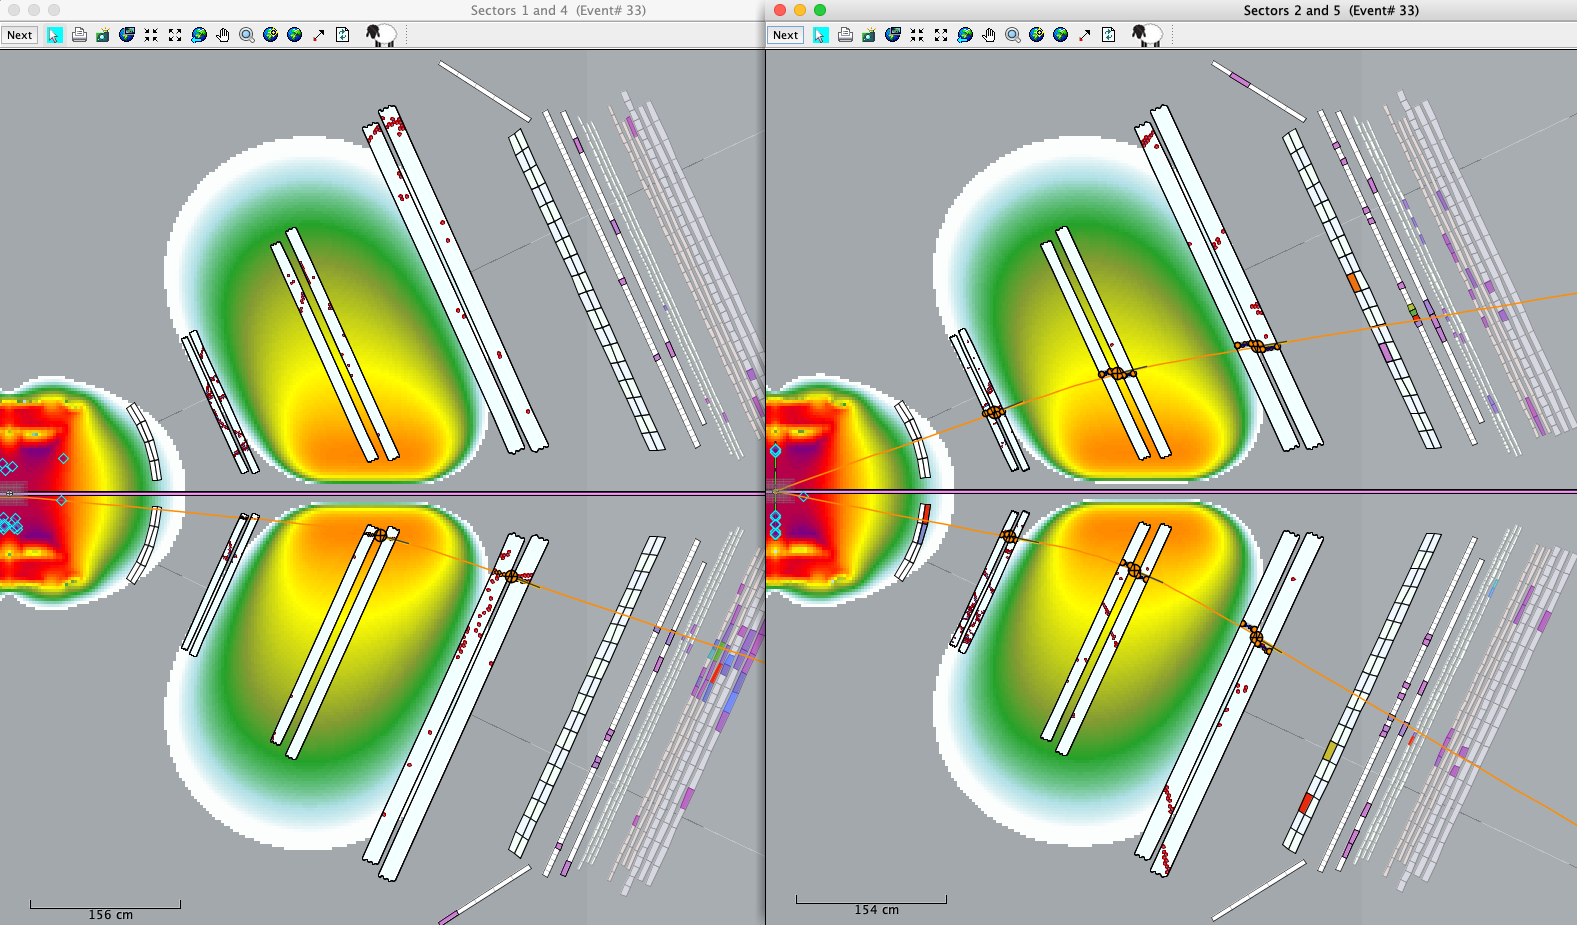
\includegraphics[width=0.95\textwidth]{pics/dcTrack3.png}
\caption{Event display of charged particle tracks in the Drift Chambers.  The reconstructed 
track in the bottom left view is an example of the use of the five-out-of-six-superlayer tracking. 
The second superlayer segment is missing in this case.  The track on the bottom right is identified 
as an electron and leaves a hit in the HTCC (red shape at the exit of the solenoid. 
}
\label{fig:dcTracks}
\end{figure*}

\subsection{Artificial Intelligence Assisted Forward Tracking}
\subsubsection{Motivation}
Recent progress in machine learning field offer a promising alternative to conventional
algorithmic tracking methods. While the conventional
methods provide algorithms that are well understood and well studied, there are some algorithms
in data reconstruction process that can be substituted with neural networks to reduce data
processing times. For CLAS12, tracking is the most time consuming process in experimental data processing.
Tracking in the DC takes up to 94\% of total data processing time, which includes finding
track candidates and iterating through track forming segments combinatorially to find the best
combinations of segments that can form a track. This time increases with luminosity as noise
segments increase and can lead to processing time degradation with higher luminosity. We have started 
to address this issue by employing machine learning techniques to find best track candidates in
each event and reduce the number of combinatorics.
\begin{figure*}
\centering
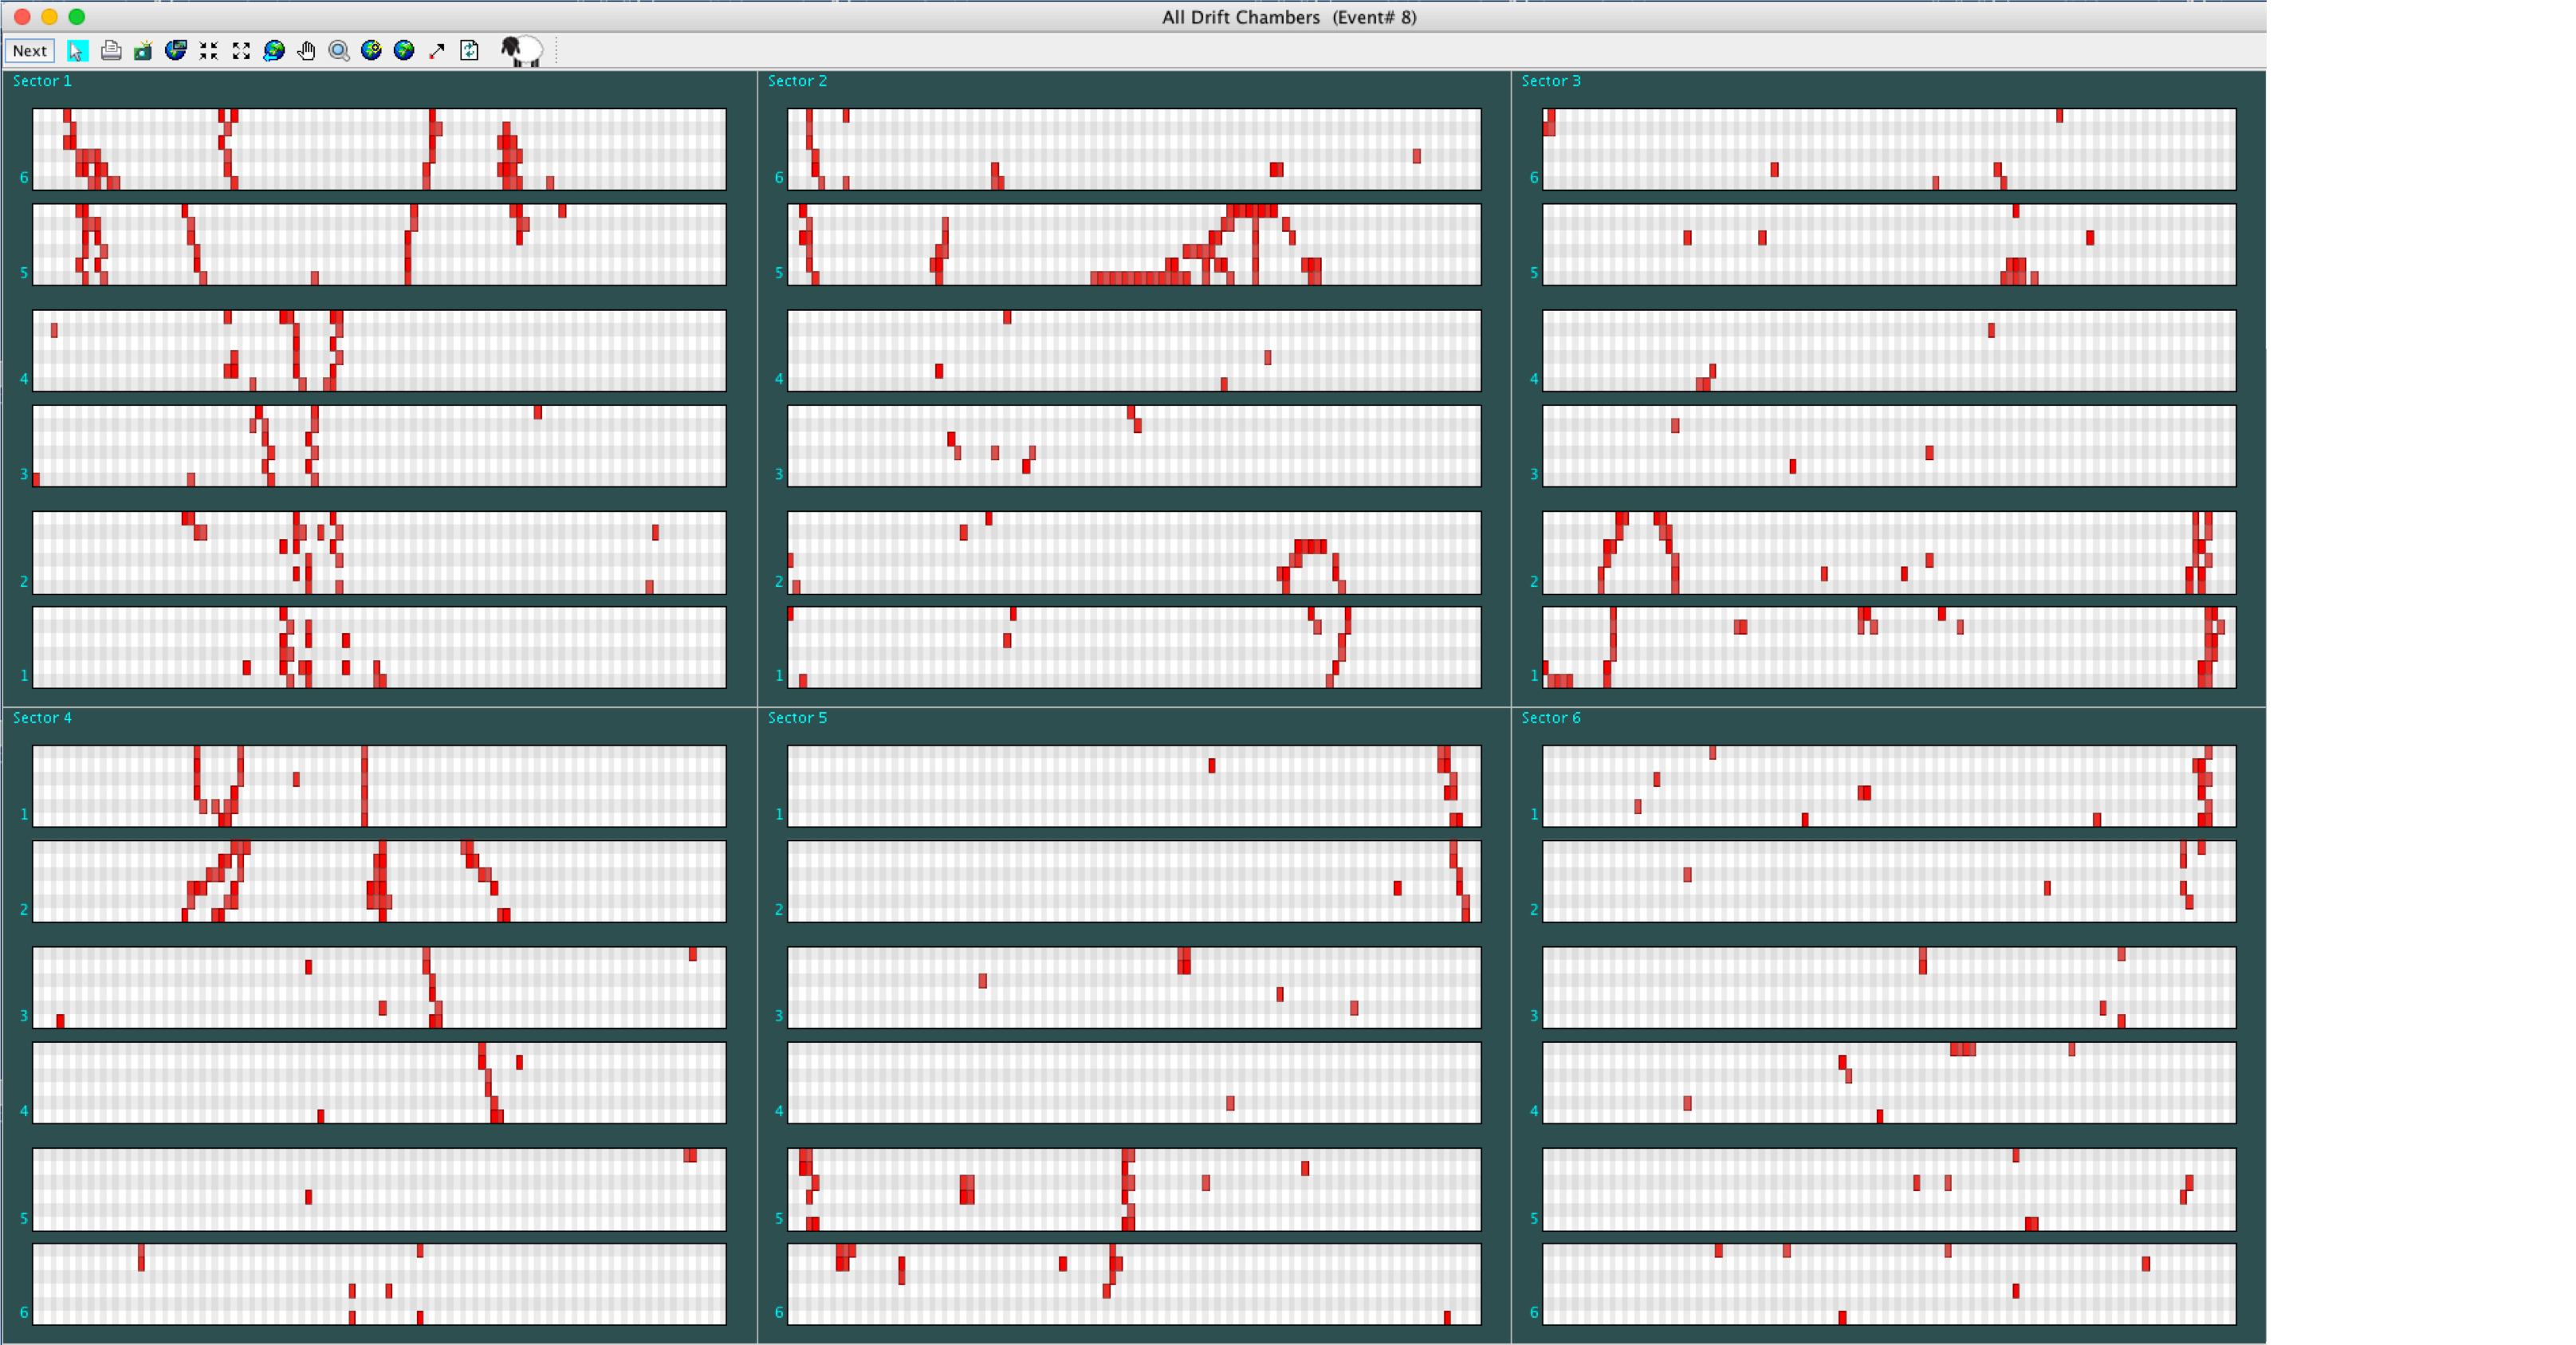
\includegraphics[width=0.95\textwidth]{pics/nn1.png}
\caption{Event display of track segments in the DC. 
}
\label{fig:nn1}
\end{figure*}
\subsubsection{Development}
With increased luminosity the number of potential DC cross candidates
increases.  This implies that the  Kalman Filter fitting algorithm must be run for all possible
combinations crosses.  Fig.~\ref{fig:nn1} shows a typical example of drift
chamber data is shown in a longitudinal projective view using CED. 
This figure illustrates the potential of combinatorial trials to identify tracks. 
We are developing a classifier convolutional neural network that can
identify which segments from each region of CLAS12 drift chambers can potentially form a
good track. We intend to use this network in reconstruction process to reduce the number of
combinatorial fitting.
Reconstructed track segments from both positive and negative tracks from the currently reconstructed data samples are used to train the Neural Network. 
We are currently testing three types of Neural Networks: boosted decision tree, multilayer perceptron, convolutional neural network.  
The accuracy of the network is measured using 4 quantities:
\begin{itemize}
\item{The ratio of valid tracks (correctly detected) to the total number of tracks in the sample. }
\item{The ratio of valid tracks and  invalid tracks (miss-predicted as valid ones; i.e. False Positives) to the total number of tracks in the sample. }
\item{The ratio of valid tracks (correctly detected with highest probability) to the total number of tracks in the sample. }
\item{The ratio of invalid tracks (False Positives) to the total number of tracks in the sample. }
\end{itemize}
Accuracy scores where determined for different training set and for the 3 types of Neural Networks studied.  Preliminary results indicated that the Convolutional Neural Network performed competitively with the Multilayer Perceptron with about 97\% accuracy and 3\% False Positives. 

The hits identified as On-Track by the Neural Network are saved in a bank and the DC reconstruction package was adapted to read these data as an input to hit-based tracking.

Benchmark results of reconstruction speed for hit-based tracking are shown in Fig.~\ref{fig:nn2}

\begin{figure}
\centering
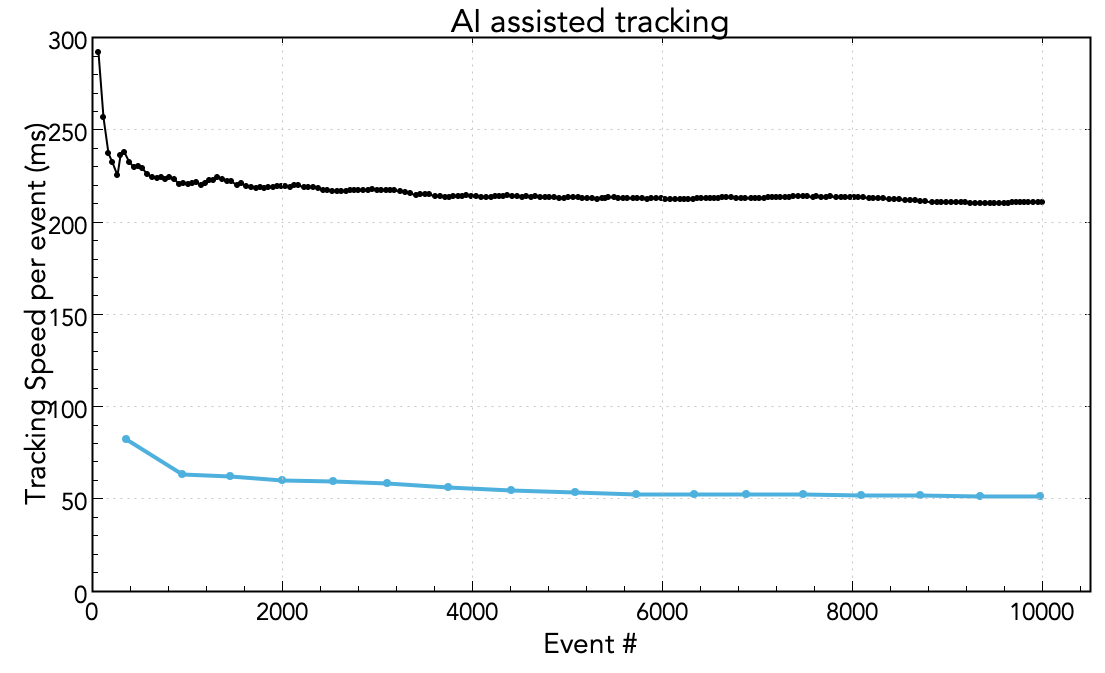
\includegraphics[width=0.5\textwidth]{pics/nn2.png}
\caption{Benchmark results of reconstruction speed for hit-based tracking.  
The (black) blue curve correspond to the (non) AI-assisted reconstruction processing time as a function of event number. 
}
\label{fig:nn2}
\end{figure}

The implementing the Neural Network software into the CLAS12 reconstruction workflow is under development. The second stage of the Machine Learning project will concentrate on efficiency improvements using AI-assisted tracking.

\subsection{Central Tracking}\label{sec:cvt}

Tracks whose angle with the beam direction is between $40^\circ$ and $135^\circ$ are reconstructed by the so called
Central Vertex Tracker (CVT). The CVT consists of twelve cylindrical layers of tracking detectors, numeroted from 1 for
the most inner layer to 12 for the most outer layer. The subset of tracking detectors forming layer 1 to 6 are silicon
strip detectors and will be referred as the Silicon Vertex Tracker (SVT) described in~\cite{svt-nim}. The layers from 7
to 12 are made of micromegas detectors and will be referred as the Barrel Micromegas Tracker (BMT) described
in~\cite{mm-nim}. The entire CVT surrounds the target and sits in a solenoid magnet able to produce a 5T-magnetic
field.

The revolution axis of the CVT coincides with the ideal beam axis which defines the z-axis of the CVT frame. The y-axis
points upward in the laboratory frame and the x-axis is defined such as the unit vectors of each axis form an direct
orthogonal basis. The origin of the CVT frame matches the center of the experimental Hall B.

An illustration of the CVT detector with CED 3-D is shown in Fig.~\ref{fig:cvt}.

\begin{figure}
\centering
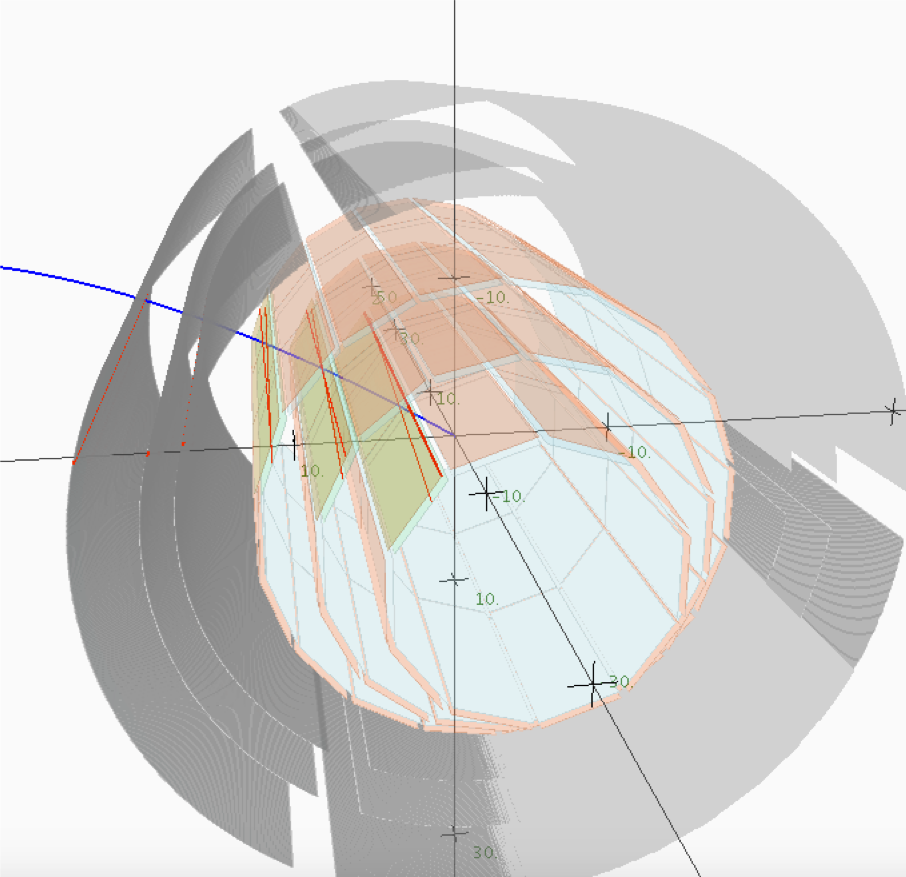
\includegraphics[width=0.5\textwidth]{pics/cvt.png}
\caption{Event display of the CVT detector. The red lines represent active SVT strips corresponding to hits on track. 
}
\label{fig:cvt}
\end{figure}

\subsubsection{Hit Clustering}
The first step of the tracking algorithm is the formation of clusters from the raw hits. The SVT raw 3-bit ADC values
are transformed into deposited charge by randomly sampling a Landau distribution fitted on test-bench data. A cluster
is a collection of contiguous hit strips. Its centroid is either given by a spatial information (a z-coordinate for
BMTC, xy-coordinates for BMTZ) or an averaged strip number for SVT. This centroid is derived by performing an average of
the relevant strip information, weighted by the maximum of the ADC pulse for micromegas strips or the equivalent
deposited charge for the SVT.
The time information associated to each hit is not used at the moment.

Before feeding all the CVT clusters to a pattern recognition algorithm, spatial coordinates must be associated to the
SVT clusters. As described in~\cite{svt-nim}, SVT layers are mechanically paired and consequently form three regions.
The readout strips of the inner and outer layer of each region make a $3^\circ$-stereo angle. By associating one
cluster of the inner layer with one cluster of the outer layer, and by assuming that an infinite momentum track crossed
perpendicularly the two layers, a preliminary candidate of the xyz-coordinates of the particle between the two layers
is derived for this cluster pair. This pairing is performed over all clusters of inner layer with all clusters of the
outer layer. Pairs whose xyz-coordinates lives outside of the SVT sensor are automatically removed from the list of
xyz-candidate list. If one of the two layer of a region has not seen the particle, then the information of the active
layer is simply ignored for the remaining of the reconstruction process.

\subsubsection{Pattern Recognition}
The trajectory of a charged particle in a solenoidal magnetic field is an helix. Because BMT detectors offers either
xy- or z-coordinates but never both, the pattern recognition cannot be performed in 3 dimensions. For particles of
large enough momentum ($p_\perp \gtrsim 0.25$ GeV/c for a 5T-solenoidal magnetic field), the xy-projection of an
helix is a circle, and the $rz$-projection is a straight line (where $r = \sqrt{x^2 + y^2}$). Therefore, a first
pattern recongition algorithm is run in xy-plane to look for circles and then a second pattern recognition algorithm is
run in rz-plane to search for straight lines.

The two pattern recognition algorithms are a modified version of the cellular automaton (CA) algorithm developed by the
Hera-B collaboration~\cite{CA-HeraB}. Here, the elementary cell of the CA is defined as a segment that connects two
2D-points.
In the $(x,y)$ plane, cells are formed with SVT and BMTZ xy-information. Two xy-clusters form a cell if the angular
distance between them is lower than a threshold. This threshold has been derived by maximizing the reconstruction
efficiency on a single track Monte-Carlo simulation with background extracted from the data. Two clusters cannot form a
cell if they are separated by more than one layer. Finally,The CA is run sector-by-sector in the BMT and, as a
consequence, a cell cannot be formed with two clusters living in different BMT sectors.
The subsequent step is the neighbor finding. A cell ``a'' is neighbor of a cell ``b'' if they share one cluster and if
the layer numbers in ``b'' are higher than the ones in ``a''. Tuned on single-track Monte-Carlo simulation without
background, cuts on the dot product between the cell directions are applied  as neighbor-forming criteria.
Now that the neighborhood of a cell is defined, the CA is evolved over $N$-evolution stage: For evolution stage $n$,
the state of all cells is updated according to $S_n = max(S_{n-1}^j) + 1$, where $S_{n-1}^j$ is the state of the
j$^{th}$-neighbor of the considered cell at evolution time $n-1$. Therefore, at evolution stage $N$, the cells with the
highest state are outer than the cells with a smalle state.
\color{red} \textbf{Caption of a figure to be produced to explain CA evolution} \color{black}

Track candidates in the $(x,y)$ plane are then formed starting from the highest state cells and following the neighbor
chain with $\Delta S = 1$. In case of multiple neighboring cells with the same state, the one that has the lower dot
product with the original cell is chosen.

Due to the poor $z$-resolution of the preliminary SVT 3D-points, the search for candidates in the $(z,r)$ plane is
performed by only using
the z-clusters of BMT. The CA algorithm trivially returns the track segments of two or three BMTC clusters.
Due to the orthogonality of the BMTC and BMTZ, all the $(z,r)$ segments of a BMT sector are combined with the $(x,y)$
candidates in the same sector. A line is fitted on the BMTC hits and its intersections with the three SVT regions are
computed. If the distance between the expected intersection and the preliminary 3D-point in the SVT region is greater
than two millimeters, then the two SVT clusters forming this preliminary point are removed from the track candidate.

\subsubsection{Track Fitting}

Each track candidate is then passed to a Kalman filter. The state vector to describe an helix is formed by five
parameters $(\varphi_0, d_0, \kappa, z_0, tan(\theta_{dip}))$, where:
\begin{itemize}
\item $d_0$ is the $(x,y)$ distance of closest approach to the CVT revolution axis,
\item $\varphi_0 = atan(p_y/p_x)$ at closest approach the the CVT revolution axis,
\item $\kappa=Q/p_\perp$ and $Q$ is the electric charge and $p_\perp=\sqrt{p_x^2+p_y^2}$,
\item $z_0$ is the distance along the $z$ axis to the CVT center,
\item and $\theta_{dip}$ is the polar angle between the track and the xy-plane.
\end{itemize}

To initialize the Kalman Filter, a first estimate of these parameters are obtained from:
\begin{itemize}
\item a circle fit in the xy-plane with SVT preliminary 3D-points and BMT xy-clusters for $d_0$, $\varphi_0$ and
$\kappa$. To improve the initialization of the fit, the point (0,0) is included in the fit with an accuracy of 100~$\mu
m$.
\item a line fit in rz-plane using only z-clusters of Micromegas to initialize $z_0$ and $\theta_{dip}$.
\end{itemize}
The covariance matrix of the two fits are merged into a 5$\times$5 matrix to initialize the covariance matrix for the
Kalman filter. Following transport equations in~\ref{ILC-Tracking}, the state vector is propagated from the CVT
revolution axis to the most outer layer of CVT, filtering at each measurement composing the track candidate. Once the
last measurement is reached, state vector and covariance matrix are brought back to the CVT revolution axis as they are
and the transport/filtering process is re-run. A maximum of five iterations is performed to make sure of the
convergence of the filtering process.

\subsubsection{Tracking Performance}

The momentum resolutions in the central and forward trackers as a function of the momentum reach
in these detectors is shown in Figs.~\ref{fig:respcvt} and~\ref{fig:respdc}, respectively.  The distributions are fit with a function of the form $\sqrt{a+b x^{2}+c/(1+d/x^{2})}$.  The resolutions achieved are well within specs and the difference in magnitude between the central and the forward trackers is due to intrinsic resolutions of these detectors.  For the forward detector, the momentum resolution in the DC is evaluated using  tracks simulated at $\theta =15\pm 5$ deg, and at $\phi = 0 \pm 5$ GeV (sample 1), to ensure that most tracks are within the sensitive volume.
Furthermore, the DC momentum resolution is correlated to the polar angle since the tracks' curvature is determined from the magnetic field intensity that is higher at lower angles in the torus field, as can be seen from Fig.~\ref{fig:restheta}, corresponding to tracks simulated at $p=4\pm 1$ GeV, $10\leq \theta\leq 25$ and $\phi = 0 \pm 5$ deg(sample 2).

These resolutions are obtained from a MC sample that does not include out of time backgrounds nor misalignments of the tracking volumes.   
A dedicated study that involves merging random background date with low luminosity data is described in [overview paper].

\begin{figure}
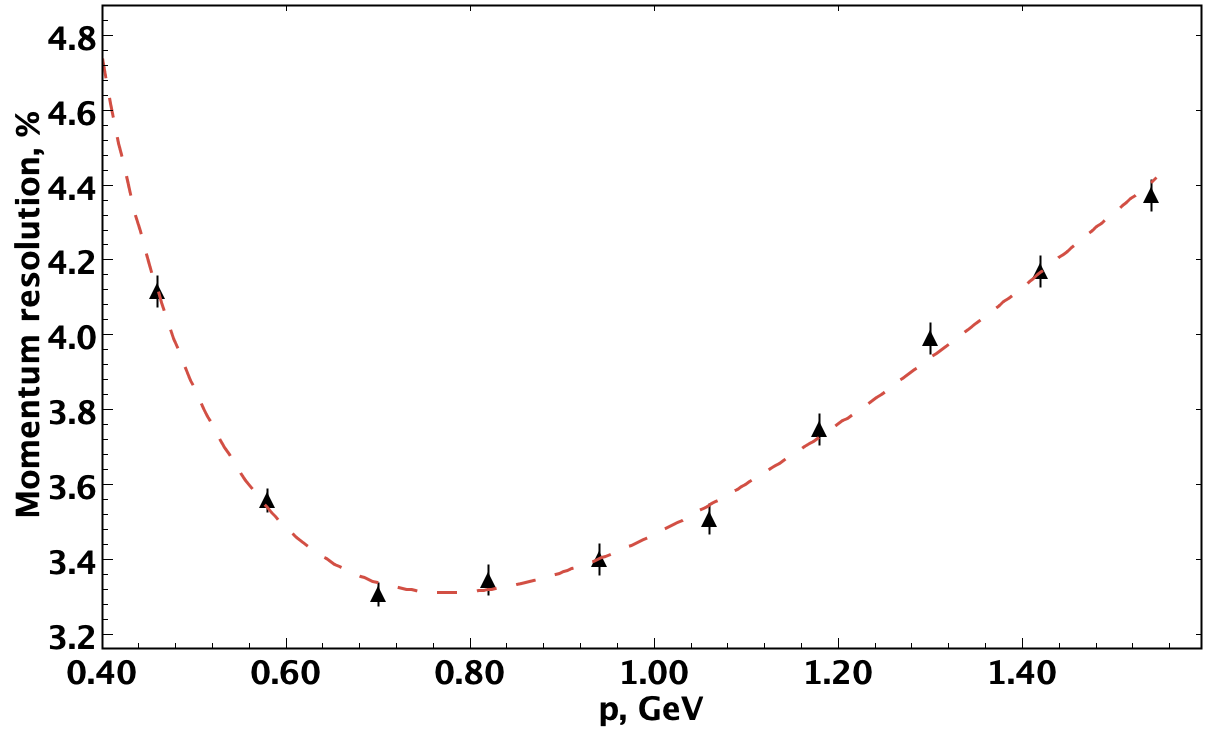
\includegraphics[width=0.45\textwidth]{pics/fddegipekmpjjiho.png}
\caption{Momentum resolution of simulated protons in the CVT.  
}
\label{fig:respcvt}
\end{figure}
\begin{figure}
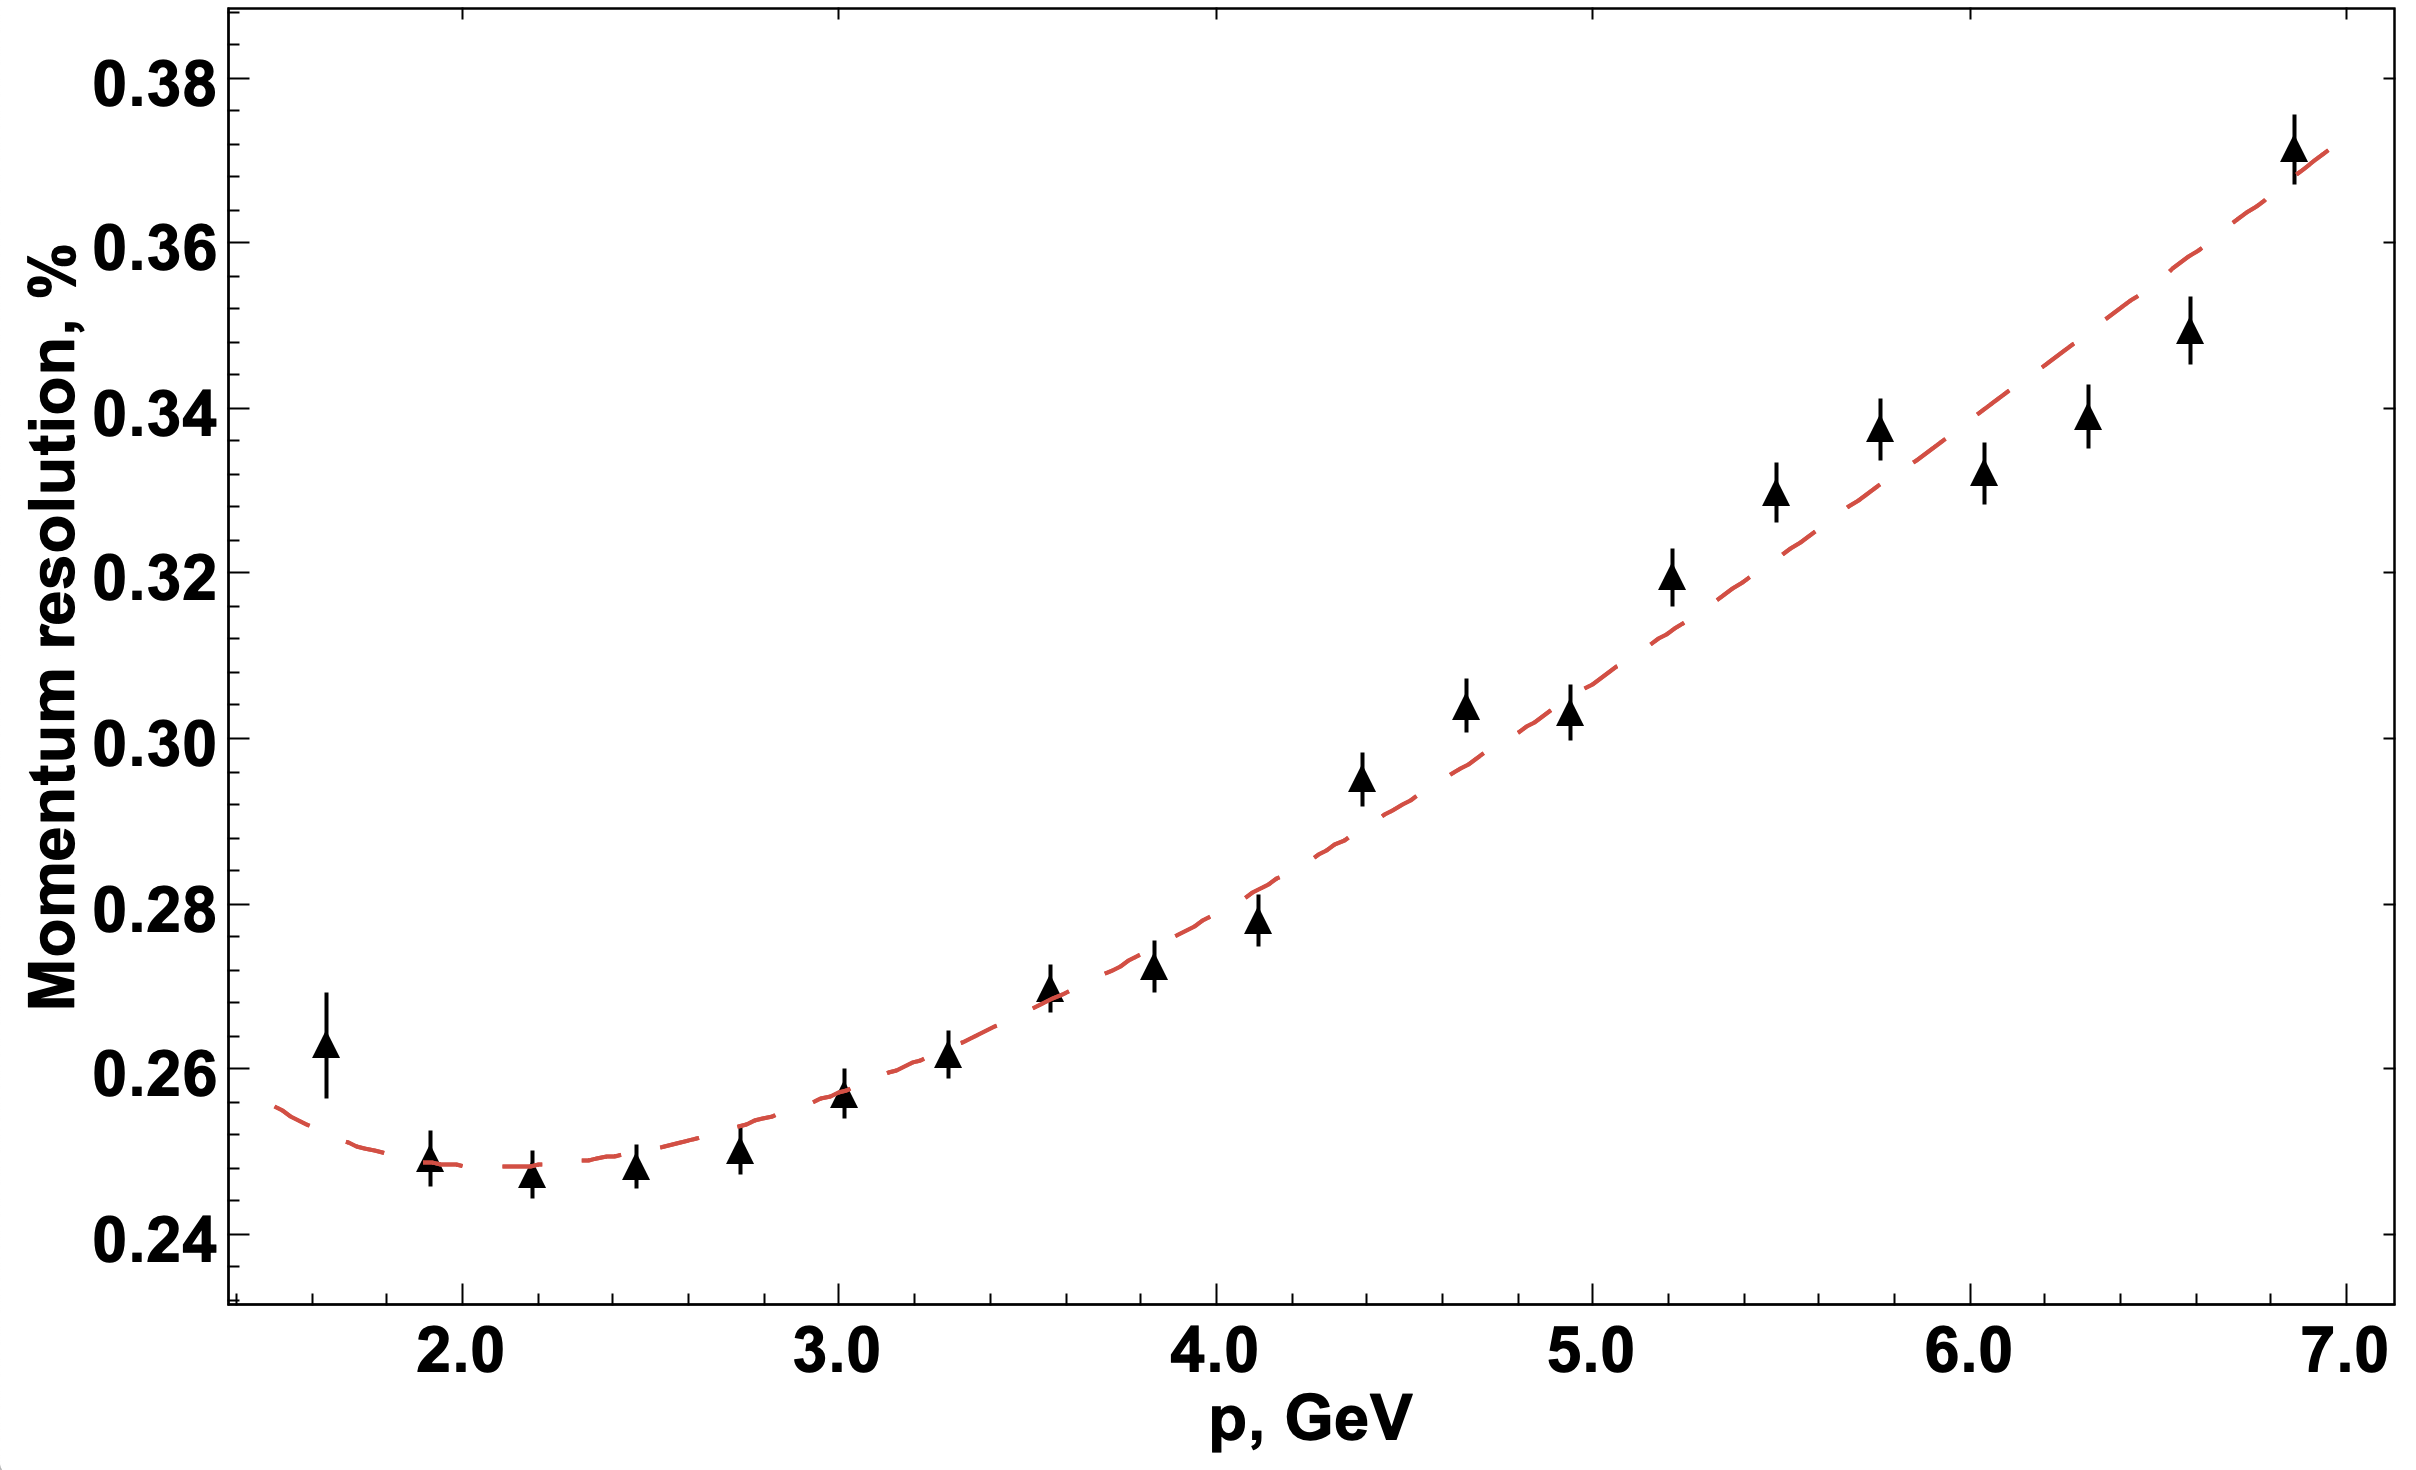
\includegraphics[width=0.45\textwidth]{pics/DCRes.png}
\caption{Momentum resolution in the DC evaluated using pions  simulated at $\theta =15\pm 5$ deg, and at $\phi = 0 \pm 5$ deg.
}
\label{fig:respdc}
\end{figure}

\begin{figure}
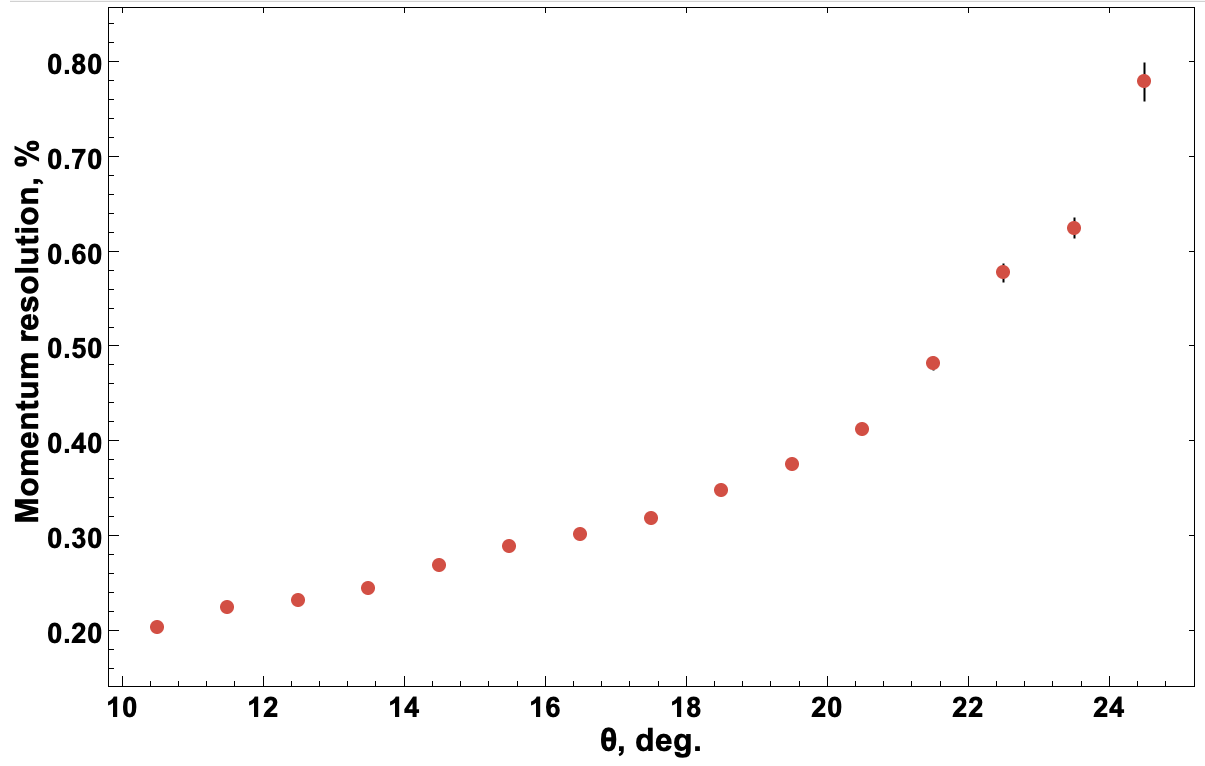
\includegraphics[width=0.45\textwidth]{pics/DCRes2.png}
\caption{Momentum resolution in the DC evaluated using  pions  simulated at $p=4\pm 1$ GeV, $10<\leq \theta\leq 25$ and $\phi = 0 \pm 5$ deg.
}
\label{fig:restheta}
\end{figure}

The tracking efficiency for in- and out-bending tracks calculated from sample 1 is shown in  Figs.~\ref{fig:trkeff}.  In-bending tracks suffer from a loss in tracking efficiency for momenta generated below 1.8 GeV at time-base level due to lack of matching with the outer detectors.  These tracks miss the sensitive volumes of the Time-of-Flight system which is required to extract time correction information needed for time-based tracking.  They do however pass the hit-base requirement.  The efficiency loss due to the afore mentioned effect can be seen by comparing the (light) blue distribution to the (dark) red one.  In the momentum range from 1.8 to 7.5 GeV, the time-based tracking efficiency is 98\%, while in the range from 1.4 to 7.5 GeV, the hit-based tracking efficiency is 99\%.  For out-bending tracks (Fig.~\ref{fig:trkeff}(bottom)), both the hit-based and time-based tracking efficiencies are flat as a function of momentum and of the order of 99\%. 


\begin{figure}
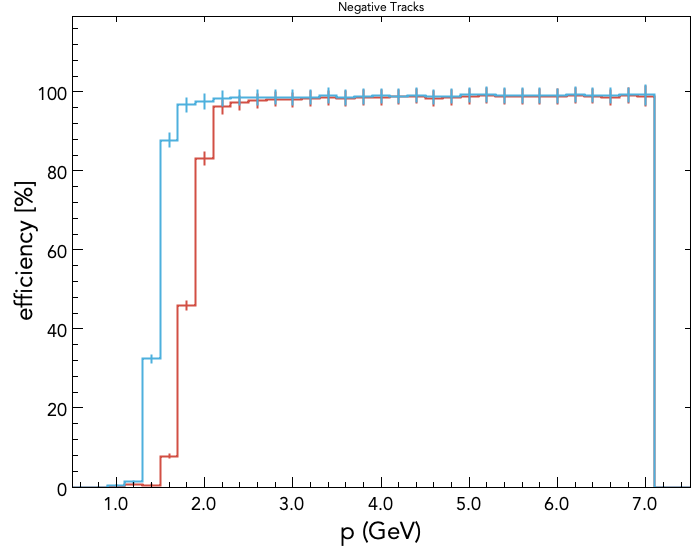
\includegraphics[width=0.45\textwidth]{pics/DCTrkgEffNegTrks.png}
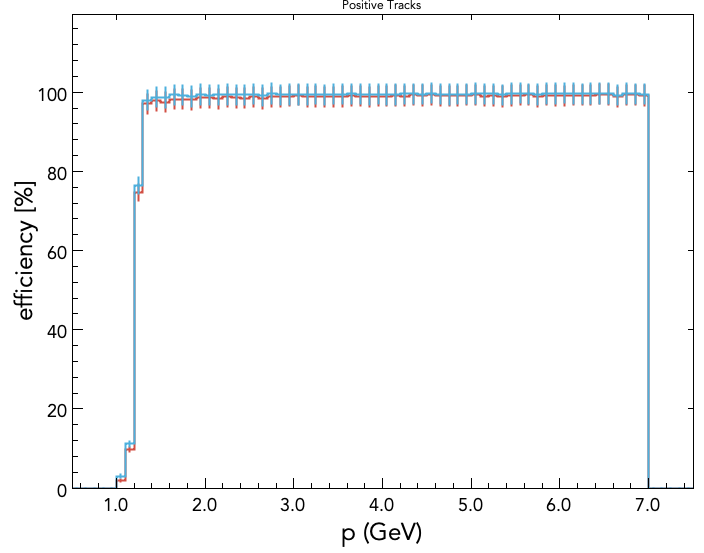
\includegraphics[width=0.45\textwidth]{pics/DCTrkgEffPosTrks.png}
\caption{DC tracking efficiency as a function of momentum evaluated using  (top) negative and (bottom) positive pions simulated at $\theta =15\pm 5$ deg, and at $\phi = 0 \pm 5$ deg. The (light) blue and (dark) red distributions correspond to the hit- and time-based tracking efficiencies, respectively.
}
\label{fig:trkeff}
\end{figure}


The polar angular dependence of the tracking efficiency obtained from sample 2 is shown in Fig.~\ref{fig:trkeffinoutb}.   The (light) green spectrum corresponds to out-bending tracks.  The efficiency is flat in the angular range from 10 to 25 deg. for outbending tracks while there is a loss of tracks below 15 deg.  As before, this is due to tracks missing the outer detectors.  

\begin{figure}
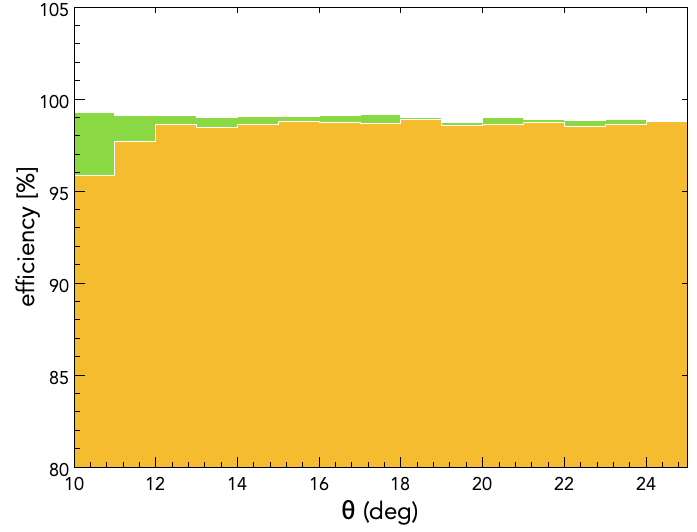
\includegraphics[width=0.45\textwidth]{pics/DCTrkEffvsThetaInandOutbenders.png}
\caption{DC tracking efficiency as a function of polar angle evaluated using  pions  simulated at $p=4\pm 1$ GeV, $10\leq \theta\leq 25$ and $\phi = 0 \pm 5$ deg.
}
\label{fig:trkeffinoutb}
\end{figure}
